% !TeX spellcheck = es_PE
% document configuration
% document class
\documentclass[10pt]{beamer}

% presentation theme
\usetheme{Madrid}

% libraries
\usepackage[spanish]{babel}
\usepackage[utf8]{inputenc} % special symbols
\usepackage{xcolor} % color
\usepackage{multicol} % multiple columns
\usepackage{multirow} % multiple rows
\usepackage{booktabs} % beautiful tables
\usepackage{graphicx, subfig} % figures
\usepackage{amsmath} % math
\usepackage{array, booktabs, tabularx}
\usepackage{animate} % animation of images
\usepackage{caption} % label
\captionsetup[figure]{font=scriptsize, justification=centering} % figure configuration
\setbeamerfont{footnote}{size=\tiny} % footnote configuration


% my colours
\definecolor{forestgreen}{HTML}{1d771d}
\definecolor{darkyellow}{HTML}{DAA520}
\definecolor{blue}{HTML}{0000FF}

% to make comment
\newcommand{\comment}[1]{}

% outline configuration
\setbeamerfont{section in toc}{size=\large}
\setbeamerfont{subsection in toc}{size=\small}
\setbeamertemplate{section in toc}[sections numbered]

% remove buttons of Madrid theme
\setbeamertemplate{navigation symbols}{}

% to remove caption from subfloat
\captionsetup[subfigure]{labelformat=empty}
\newcommand{\figcolor}{\textcolor{blue}{Figura: }}

%\newcommand{\mcx[1]}{\multicolumn{1}{>{\centering\arraybackslash}X}{\textbf{#1}}}	



% introduction parameters
\title[Laboratorio 0]{Control no lineal}
\subtitle{\textbf{Introducción a los módulos de control y Simulink}}

\author[J. Charaja and R. Terreros (UTEC)]{\textbf {Profesora} \\ Ruth Canahuire \\ \vspace{1em} \textbf{Asistentes de enseñanza} \\ Jhon Charaja y Ricardo Terreros}

\logo{
\includegraphics[height=8em]{imgs/utec-logo.png}}

\date{\today}


\begin{document}
\graphicspath{{imgs/}}
\frame{\titlepage}
% primer slide
% describir los componentes del módulo de control (QUBE-Servo 2) y cómo lo vamos a usar
% una foto de la placa de conexiones, una foto de cubo (enfocar conexión), una foto del péndulo y una foto del disco de masa

% segundo slide:
% mostrar como conectar el módulo, imágen de las conexiones (placa -> módulo) y una imágen del cubo con el péndulo y disco de masa

% tercer slide:
% indicar cúales son los bloques de Quanser para recibir data (posición) y enviar data (señal de control)

% cuarto slide
% mostar el diagrama de bloques de control de posición en Simulink .

% quinto slide
% controlar velocidad

\section{Introducción}

\begin{frame}
\frametitle{Módulos del laboratorio}

     \begin{figure}
     	\subfloat[\figcolor caja de control con tarjeta QFLEX 2 USB]{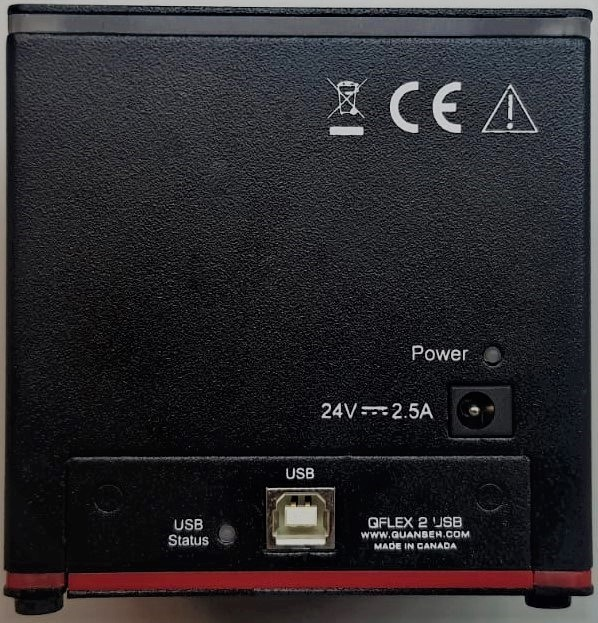
\includegraphics[height=0.4\textheight]{qube.jpeg}}
     	\hfill
      	\subfloat[\figcolor módulo de péndulo invertido]{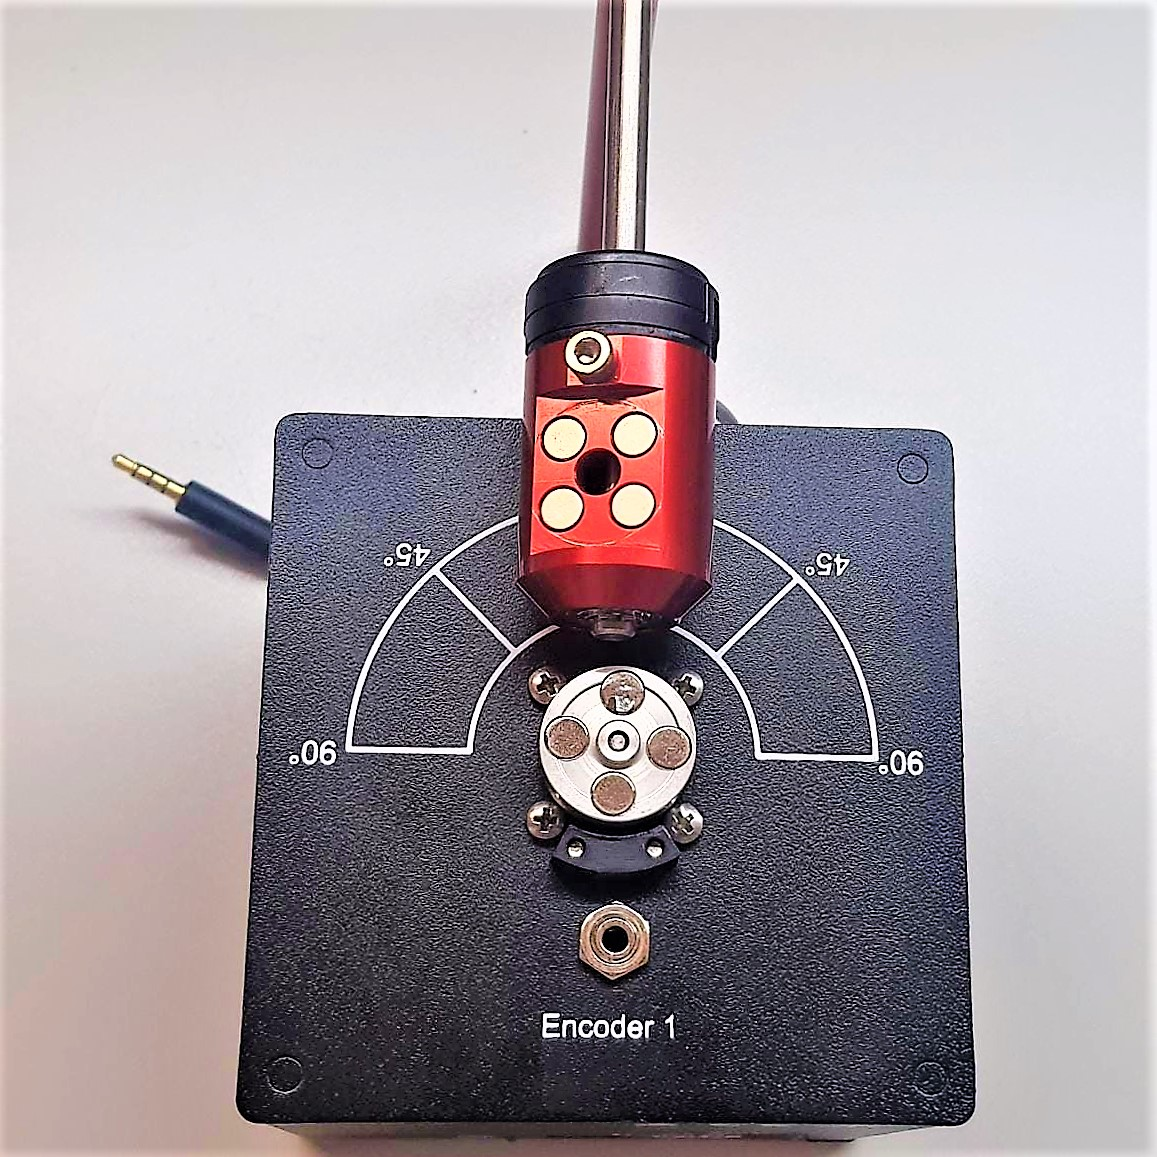
\includegraphics[height=0.4\textheight]{qube_pendulum.jpeg}} 
      	\hfill
      	\subfloat[\figcolor módulo de carga lineal]{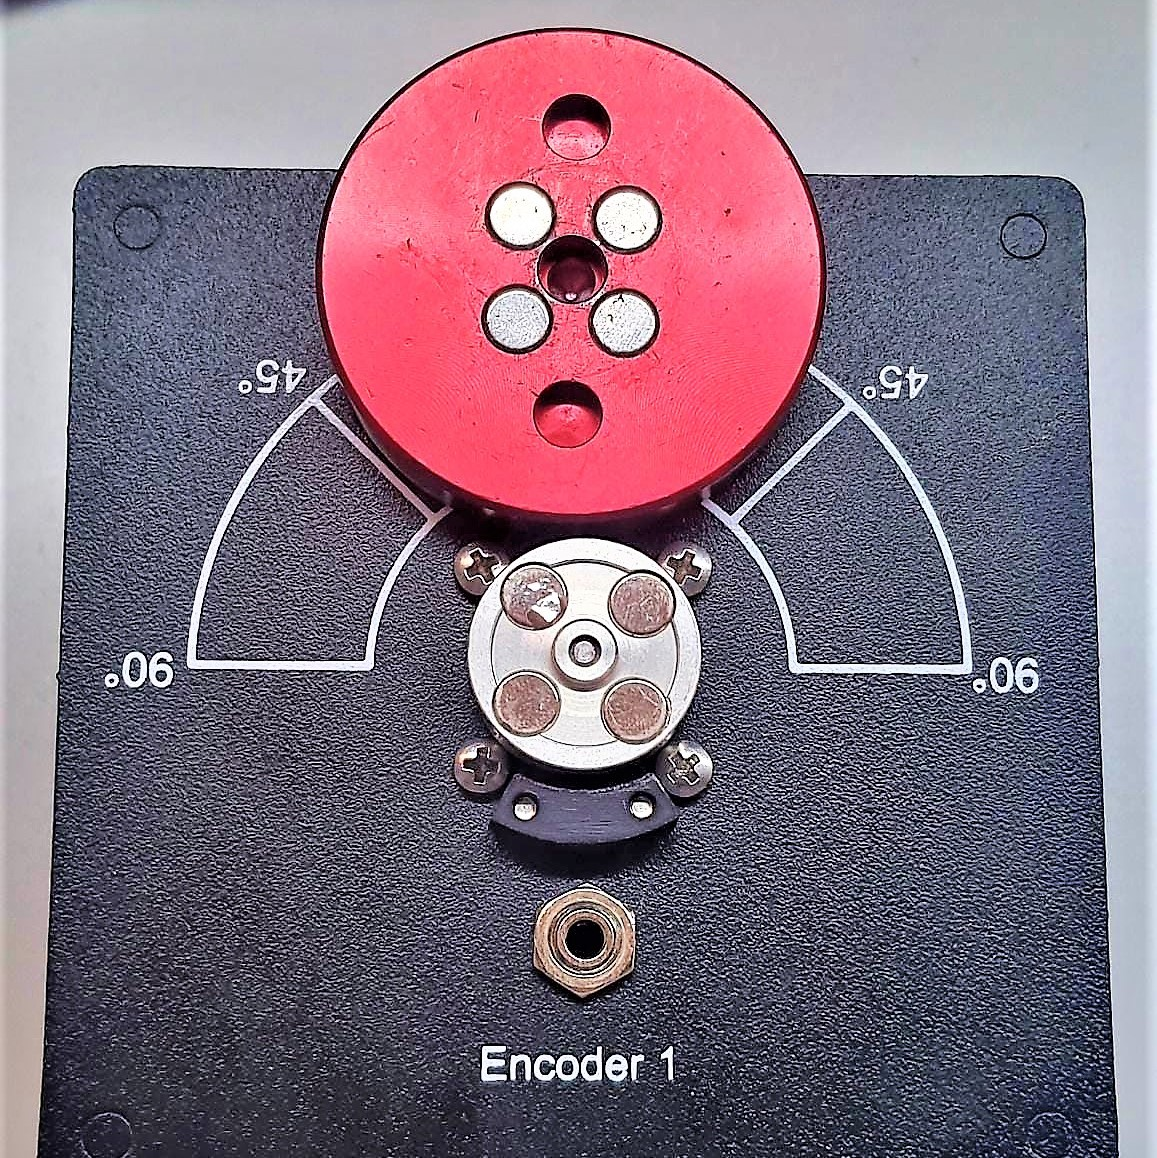
\includegraphics[height=0.4\textheight]{qube_disk.jpeg}}  
     \end{figure}
     	  
\end{frame}
	
\begin{frame}
\frametitle{Bloques de Quanser en Simulink}
	
     \begin{figure}
     	\subfloat[\figcolor módulo de control]{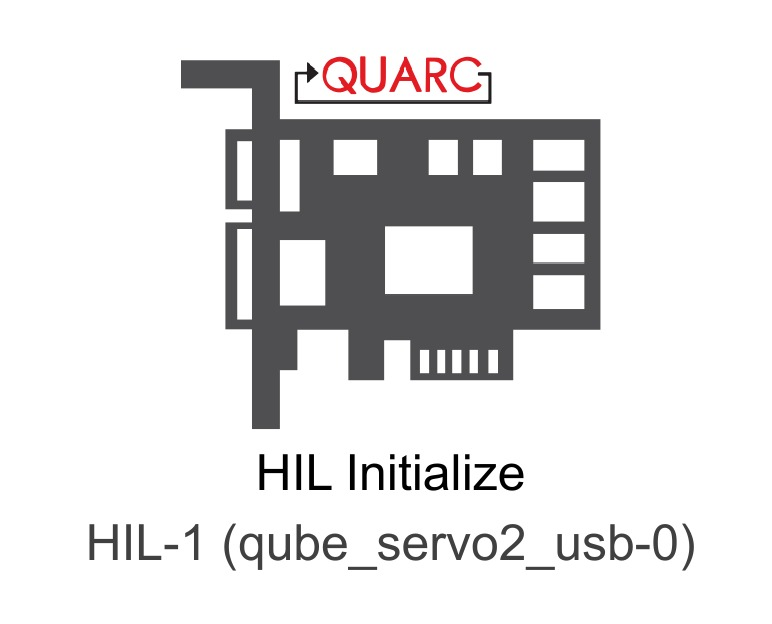
\includegraphics[height=0.35\textheight]{quanser_modulo.jpeg}}
     	\hfill
      	\subfloat[\figcolor recibir posición angular del motor]{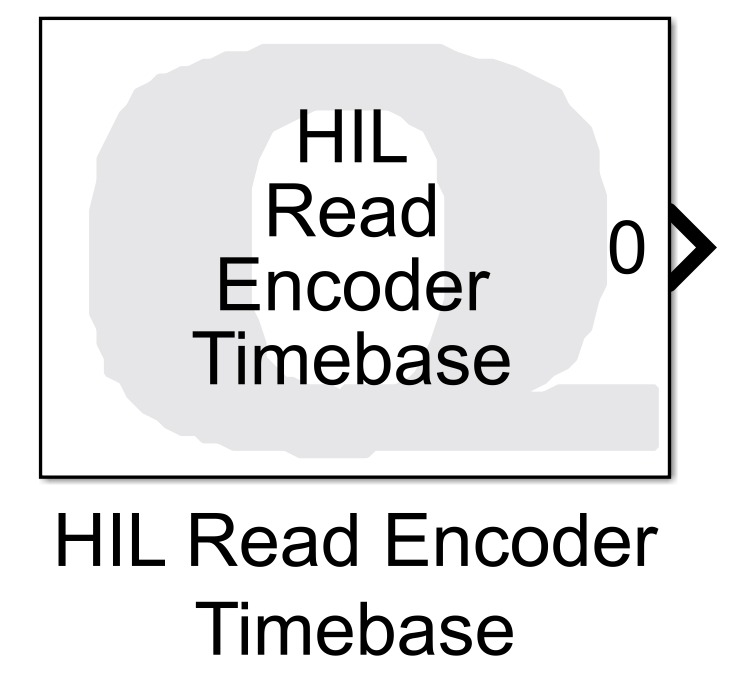
\includegraphics[height=0.35\textheight]{quanser_read.jpeg}} 
      	\hfill
      	\subfloat[\figcolor enviar señal de control]{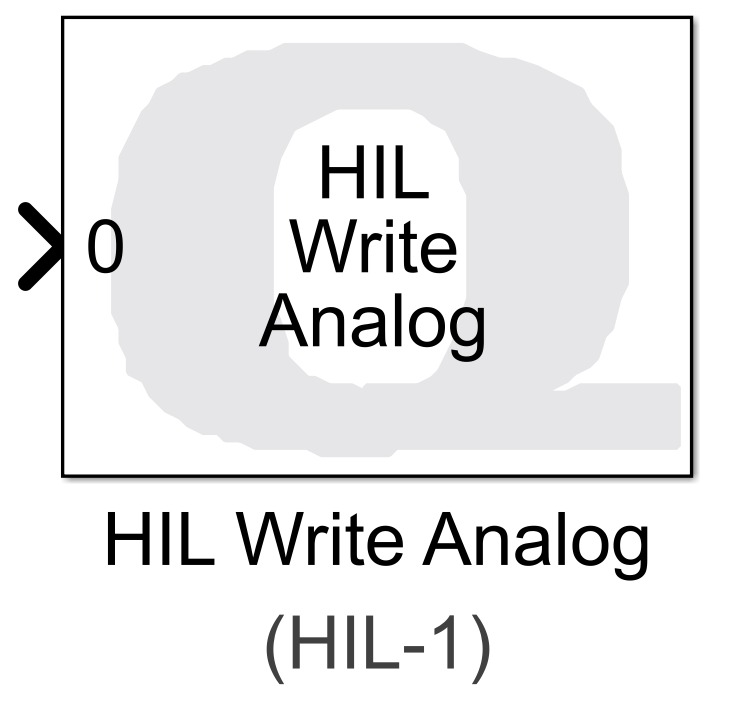
\includegraphics[height=0.35\textheight]{quanser_write.jpeg}}  
     \end{figure}
\end{frame}

\begin{frame}
\frametitle{Diagrama de Simulink: módulo con carga lineal}
\begin{figure}
\centering
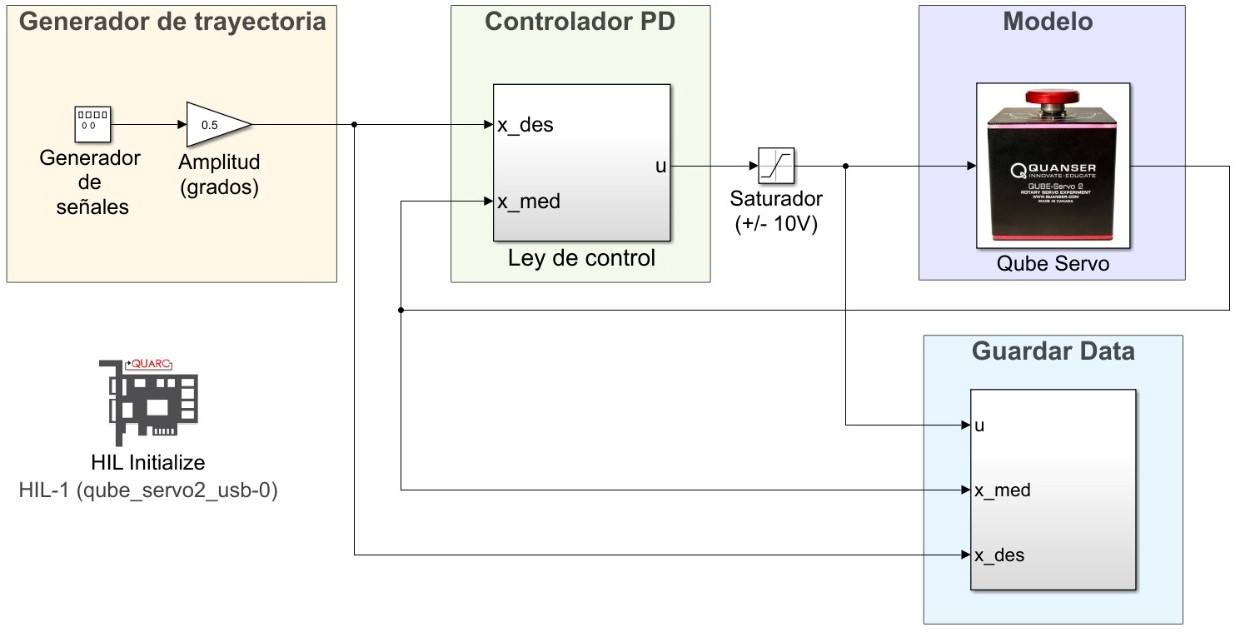
\includegraphics[width=0.95\textwidth]{simulink_qube_disk.jpeg}
\end{figure}

\end{frame}

\begin{frame}
\frametitle{Diagrama de Simulink: módulo con péndulo invertido}
\begin{figure}
\centering
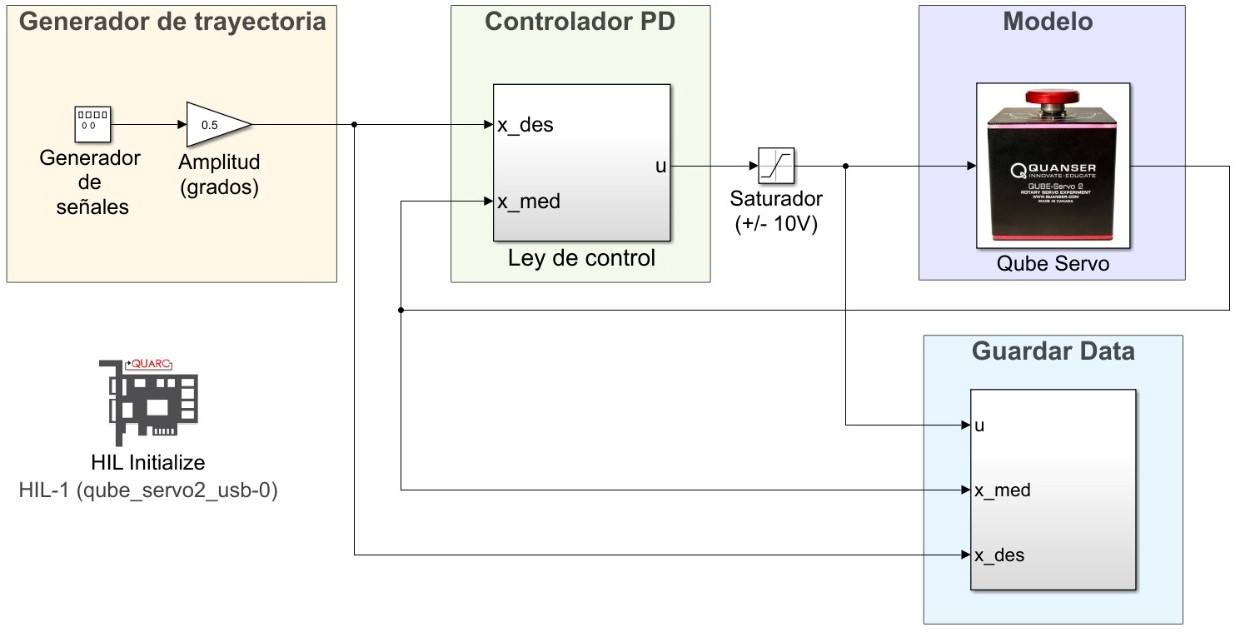
\includegraphics[width=0.95\textwidth]{simulink_qube_disk.jpeg}
\end{figure}

\end{frame}

\end{document}